\documentclass[12pt,fleqn]{article}
\setlength{\parindent}{0pt}
\usepackage{graphicx}
\usepackage{cancel}
\usepackage{listings}
\usepackage[latin5]{inputenc}
\usepackage{color}
\setlength{\parskip}{8pt}
\setlength{\parsep}{0pt}
\setlength{\headsep}{0pt}
\setlength{\topskip}{0pt}
\setlength{\topmargin}{0pt}
\setlength{\topsep}{0pt}
\setlength{\partopsep}{0pt}
\setlength{\mathindent}{0cm}

\begin{document}
Ders 23

Akis (Flux)

Aslinda akis cizgisel entegrallerin degisik bir seklidir. Diyelim ki $C$
egrisi ve $\vec{F}$ vektor alani var, o zaman $C$ uzerinden $\vec{F}$'in
akisi 

\[ \int_C \vec{F} \cdot \hat{n} \ ds \]

olarak gosterilir. Simdi bu entegral icindeki ogelerin ne oldugunu tarif
edelim. 

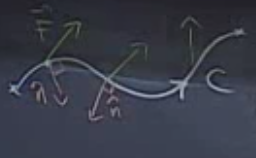
\includegraphics[height=3cm]{23_1.png}

$\hat{n}$ = $C$ egrisine dik olan birim normal vektordur, $\vec{T}$'ye 90
derece saat yonunde diktir. Saat yonunde dedik cunku mesela ustteki resimde
en soldaki $\hat{n}$ yukari da isaret ediyor olabilirdi, onu degil, asagi
dogru gideni sectik.

Entegral neyi hesaplar? Egri uzerindeki her noktada, vektor alani ile ayni
egrinin normalleri ile yapilan carpimlarin toplamini. Yani $C$'yi en ufak
parcalar $\Delta s$'lere ayirinca 

\[ Akis = \lim_{\Delta s \to 0} 
\bigg( \sum \vec{F} \cdot \hat{n} \ \Delta s \bigg) \]

Bu kavrami daha once hesapladigimiz ``yapilan is'' karsilastirmak
gerekirse

\[ Is = \int_C \vec{F} \cdot d\vec{r} = \int_C \vec{F} \cdot \vec{T} \ ds \]

Isi hesaplarken her noktada $\vec{F}$'in egri $C$'nin tegetine yansimasini
hesapliyorum. 

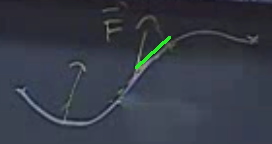
\includegraphics[height=2cm]{23_2.png}

Yani egri uzerinde hareket ederken ``$\vec{F}$ ile ne kadar birlikte, ne
kadar ona ters sekilde'' hareket edildiginin hesabi yapilan isi veriyor. 

Kiyasla akis hesabi, egri uzerinde hareket ederken $\vec{F}$'in egrinin
``ne kadar icinden gectiginin'' hesabi. Ruzgarli bir havada bir yolda
yuruyorum, akis ruzgarin bana ne kadar yandan carptigini gosteriyor. Akis
hesabi bu carpis saga dogru olunca onu pozitif, saga dogru olunca onu
negatif olarak hesaplar. 














\end{document}
